\Underline{Note!} In this case we have
\[\Braket{\Creab_{\v{q}}\Annib_{\v{q}}}\neq\dfrac{1}{e^{\beta\omega_{\v{q}}}-1}.\]
Instead we find, using equation~\eqref{eq:n_a}:
\[\Braket{\Creab_{\v{q}}\Annib_{\v{q}}}=v_{\v{q}}^2+\left(u_{\v{q}}^2+v_{\v{q}}^2\right)\dfrac{1}{e^{\beta\omega_{\v{q}}}-1}.\]
This means that we can write $\Ma_\text{A}$ as
\[\Ma_\text{A}=N_\text{A}S-\Sum_{\v{q}}\left[v_{\v{q}}^2+\left(u_{\v{q}}^2+v_{\v{q}}^2\right)\dfrac{1}{e^{\beta\omega_{\v{q}}}-1}\right].\]
\textcolor{red!80!black}{\emph{(...) dependent correction (...),}}
\[\tanh(2\theta)=\dfrac{2\gamma_{\v{q}}}{z}=\dfrac{2\tanh(\theta)}{1+\tanh^2(\theta)},\]
where $z=2d$ on a \Underline{cubic} $d$-dimensional lattice.
\[\tilde{\gamma}_{\v{q}}\equiv\dfrac{2\gamma_{\v{q}}}{z}=\dfrac{1}{d}\Sum_{\alpha=1}^d\cos(q_\alpha),\]
or by defining
\[t\equiv\tanh(\theta),\qquad s\equiv\sinh(\theta),\qquad c\equiv\cosh(\theta),\]
\[\tilde{\gamma}_{\v{q}}=\dfrac{2t}{1+t^2}\qquad\Rightarrow\qquad\tilde{\gamma}_{\v{q}}^2=\dfrac{4t^2}{(1+t^2)^2}=\dfrac{4s^2c^2}{(c^2+s^2)^2}.\]
Remember: $c^2-s^2=1$, which means that
\[\tilde{\gamma}_{\v{q}}^2=4\dfrac{s^2(1+s^2)}{(1+2s^2)^2}.\]
We now introduce $x\equiv s^2$ and $b\equiv\tilde{\gamma}_{\v{q}}^2/4$:
\[b=\dfrac{x(1+x)}{(1+2x)^2}\qquad\xRightarrow{\;x>0\;}\qquad x=-\dfrac{1}{2}+\dfrac{1}{2}\,\dfrac{1}{\sqrt{1-4b}}.\]
This means that we find
\[\sinh^2(\theta)=v_{\v{q}}^2=\dfrac{1}{2}\left(\dfrac{1}{\sqrt{1-\tilde{\gamma}_{\v{q}}^2}}-1\right),\qquad u_{\v{q}}^2=1+v_{\v{q}}^2=\dfrac{1}{2}\left(\dfrac{1}{\sqrt{1-\tilde{\gamma}_{\v{q}}^2}}+1\right).\]
Combining these results:
\[\boxed{u_{\v{q}}^2+v_{\v{q}}^2=\dfrac{1}{\sqrt{1-\tilde{\gamma}_{\v{q}}^2}}.}\]
As was shown in assignment 3,
\[\omega_q=4|J|Sd\left(1-\tilde{\gamma}_{\v{q}}^2\right)^2.\]
For a $d$-dimensional ``cubic'' lattice we can write
\[\begin{array}{r@{\;}c@{\;}l}
	\tilde{\gamma}_{\v{q}}							& =			& \dfrac{1}{d}\left(d-\dfrac{\v{q}^2}{2}+\cdots\right)=1-\dfrac{\v{q}^2}{2d}+\cdots,\\\\
	\tilde{\gamma}_{\v{q}}^2						& \approx	& 1-\dfrac{\v{q}^2}{d}+\cdots,\\\\
	1-\tilde{\gamma}_{\v{q}}^2						& =			& \dfrac{\v{q}^2}{d}+\cdots,\\\\
	\dfrac{1}{\sqrt{1-\tilde{\gamma}_{\v{q}}^2}}	& =			& \dfrac{\sqrt{d}}{|\v{q}|}+\cdots=u_{\v{q}}^2+v_{\v{q}}^2.\qquad(|\v{q}|\ll1.)
\end{array}\]
Substituting this back, we get
\[\omega_{\v{q}}=4|J|S\sqrt{d}|\v{q}|\]
when $|\v{q}|\ll1$, which in the case of $d=2$ is in agreement with equation~\eqref{eq:omega_ferromagnetic}. The temperature-dependent correction to the magnetization can now be calculated:
\[\begin{array}{r@{\;}c@{\;}l}
	\Delta\Ma(T)	& =			& -\Sum_{\v{q}}\left(u_{\v{q}}^2+v_{\v{q}}^2\right)\dfrac{1}{e^{\beta\omega_{\v{q}}}-1}\\\\
					& \approx	& -\Sum_{\v{q}}\dfrac{\sqrt{d}}{|\v{q}|}\dfrac{1}{e^{\beta|J|\eta|\v{q}|}-1}\qquad\text{(Low T.)}\\\\
					& =			& -\beta\Omega_d\Int_0^\infty d|\v{q}|\,\dfrac{|\v{q}|^{d-2}}{e^{\beta|J|\eta|\v{q}|}-1}.
\end{array}\]
Making a change of variables by introducing
\[x=\beta|J|\eta|\v{q}|,\]
the integral is evaluated as
\[\Delta\Ma(T)\propto\left(\dfrac{1}{\beta|J|\eta}\right)^{d-2+1}\Int_0^\infty dx\,\dfrac{x^{d-2}}{e^x-1}\propto\left(\dfrac{T}{|J|}\right)^{d-1}.\]
In the case where $d=3$ this means that
\[\Delta\Ma(T)\propto\left(\dfrac{T}{|J|}\right)^2\qquad\text{(\Underline{Antiferromagnetic})}.\]
Recall the ferromagnetic case, in which for $d=3$ we got (\textcolor{red!80!black}{equation reference needed})
\[\Delta\Ma(T)\propto\left(\dfrac{T}{|J|}\right)^{3/2}.\]
Comparing the two, we can say that
\begin{figure}
	\centering
	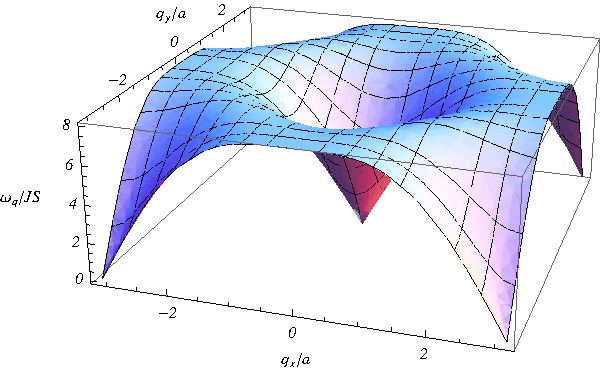
\includegraphics{img/omega_antiferromagnetic_compress}
	\caption{\label{fig:omega_antiferromagnetic_compress}The angular frequency $\omega_{\B{q}}$ as a function of the momentum $\B{q}$ for the antiferromagnetic case described by equation~\eqref{eq:omega_antiferromagnetic}.}
\end{figure}
\[\Delta\Ma_{\text{AF}}(T)=\Delta\Ma_{\text{Ferro}}(T)\cdot\left(\dfrac{T}{|J|}\right)^{1/2}\ll\Delta\Ma_{\text{Ferro}}(T).\qquad(T/J\ll1.)\]
The corrections to $\Ma$ due to \Underline{temperature effects} are weaker in antiferromagnets than in ferromagnets. This can be seen from the magnon spectrum (compare figures~\ref{fig:omega_ferromagnetic_compress} and~\ref{fig:omega_antiferromagnetic_compress}). It is \Underline{easier} to thermically excite ferromagnetic magnons than antiferromagnetic ones. We thus find a bigger temperature correction for the magnetization in a ferromagnet than in an antiferromagnet.

\Underline{But!} Note that ferromagnets don't have quantum fluctuations, while antiferromagnets do.